\subsection{Effective Field of View}

To determine a camera’s field of view, we specify the ground plane within 
an image and adjust the polygon to discard occluded areas. 
We obtain the camera's effective field of view by transforming the vertices
into the shared top view (Figure \ref{fig:fov}). Repeating this process 
for each camera allows to map the collective coverage of the CN.

\begin{figure}[t]
	\centering
	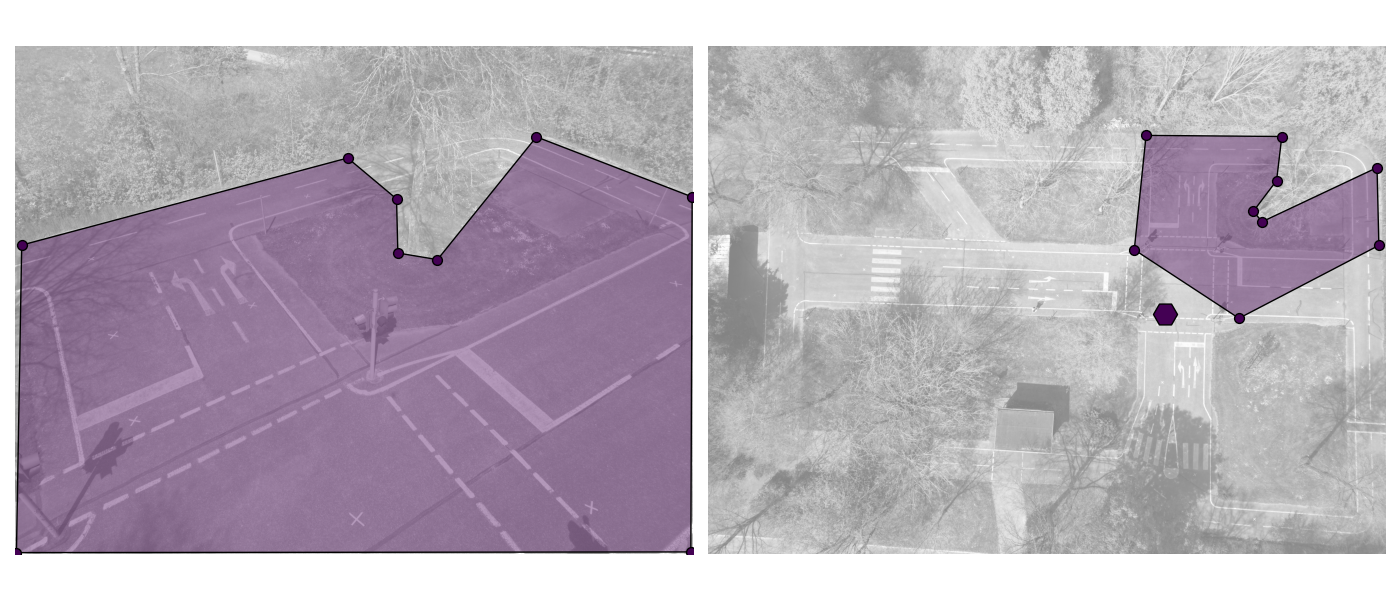
\includegraphics[width=0.45\textwidth]{figures/predicted_fov.png}
	\caption{Example for one camera (IMG\_01): Transforming an effective field 
	of view into the top view. The hexagon shows the camera's position.}
	\label{fig:fov}
\end{figure}

